\chapter{Time-Domain Representation of Discrete-time Signals}

\textbf{Time domain} refers to the analysis of mathematical functions, physical
signals or time series of economic or environmental data, with respect to
\emph{time}. In the time domain, the signal or function's value is known for
all real numbers, for the case of continuous time, or at various separate
instants in the case of discrete time. An oscilloscope is a tool commonly used
to visualize real-world signals in the time domain. A time-domain graph shows
how a signal changes with time, whereas a fre\-quen\-cy-do\-ma\-in graph shows
how much of the signal lies within each given frequency band over a range of
frequencies.

Though most precisely referring to time in physics, the term time domain may
occasionally informally refer to position in space when dealing with spatial
frequencies, as a substitute for the more precise term spatial domain~\cite{bib:wikiTimeDomain}.

\section{Signal definition}

In signal processing, a \textbf{signal} is a function that conveys information
about a phenomenon. Signals are functions of independent variables, such as
\emph{time}, \emph{distance}, \emph{position}, and so on. They are represented
as se\-quen\-ces of numbers, called \emph{samples}. Signals are composed of
samples---the single values of the signal at a certain, discrete time quantum $n
\in \Z$. Signals will be denoted with $\{x[n]\}$ while samples will be denoted
as $x[n]$. The variable $n$ may or may not be an integer, since the quantum of
time may not be constant in some applications.

Typically a discrete signal can be either a \emph{sampled-data signal} or a
\emph{digital} signal. Both types of signals only exist in specific time quanta
and they are likely the result of a sampling, but only digital signals have
\emph{quantized} value---common sampled-data signals will possess continuous
values. Values of digital signals are usually obtained from sample values
either by \emph{rounding} or \emph{truncation} techniques---in both cases an
error occurs.

Since signals can have multiple time domains, one has to clarify when
equivalences between amplitudes may apply. In particular, the following
relationship \[ x[n] = \left.x_a(t)\right|_{t=nT} = x_a(nT), n \in \Z\]
yields only as long as we do not take in account any \emph{quantization error},
since---by definition---digital signals are the result of both a sampling process
and a quantization process. The spacing between two samples is said to be
\emph{sampling interval} or \emph{sampling period} and measures in seconds,
and the reciprocal of such quantity is called \emph{sampling frequency} $F_T$
or $F_S$ and measures in Hertz.

\section{Basic signal properties}

\subsubsection{Nature of signals}

Signals can be either \emph{deterministic} or \emph{random}; the first case
denotes a signal that can be inferred by some rule or formula, while a random
signal cannot be generally predicted ahead of time. Examples of random signals
are the \emph{stock exchange}, or the \emph{coin flip}. Random signals are
usually considered as they are generated in a random fashion---even though
there might exist some actual underlying rule we don't actually know.

\subsubsection{Filters}

A \emph{filter} is a system which \emph{is able to control the frequency
content of the output with respect to the input signal}. When a filter is
\emph{linear}, the output of the filtering operation sums up to the
\emph{convolution} operation, which is the following signal,
\[
y(t) = \int_0^T x(t - \tau)h(\tau)d\tau.
\]
The role of $\tau$ in the convolution is to shift-reverse one of the two
signals, while the multiplication with the other signal occurs. This ensures
that the overall result will be a new signal which is the sum,
sample-to-sample, between one of the two signals in its original form and a
``moving'' shift-reversed form of the other one.

\subsubsection{Visual representation of a signal}

A signal can be also represented as a se\-quen\-ce of values inside brackets. To
denote where the time instant $0$ is, an arrow is placed below the sample of the
se\-quen\-ce corresponding to $n=0$. As an example, the following notation can express a signal:
\[ \{x[n]\} = \{\dots, -0.2,1,\underset{\uparrow}{3},-6.7,-5.4,0.1,3.6,1.2,\dots\}\] and, with this notation, $x[0]=3$.

To represent signals, a \emph{stem plot} is usually adopted. There are two
different forms of stem plot: a first one in which only samples are
represented---dots along with their straight vertical line denoting the
\emph{amplitude} of the signal in such quantum of time---and another one in
which superposed to the samples an analog-like line is represented. In the
latter case, there may be two different interpretations; either the digital
signal is sampled from an original analog signal, or the continuous line
denotes the amplitude of the digital signal \emph{as if} it were analog.

\begin{figure}[ht]
\begin{center}
\scalebox{0.6}{
% Title: gl2ps_renderer figure
% Creator: GL2PS 1.4.2, (C) 1999-2020 C. Geuzaine
% For: Octave
% CreationDate: Wed Oct 19 08:50:18 2022
\setlength{\unitlength}{1pt}
\begin{picture}(0,0)
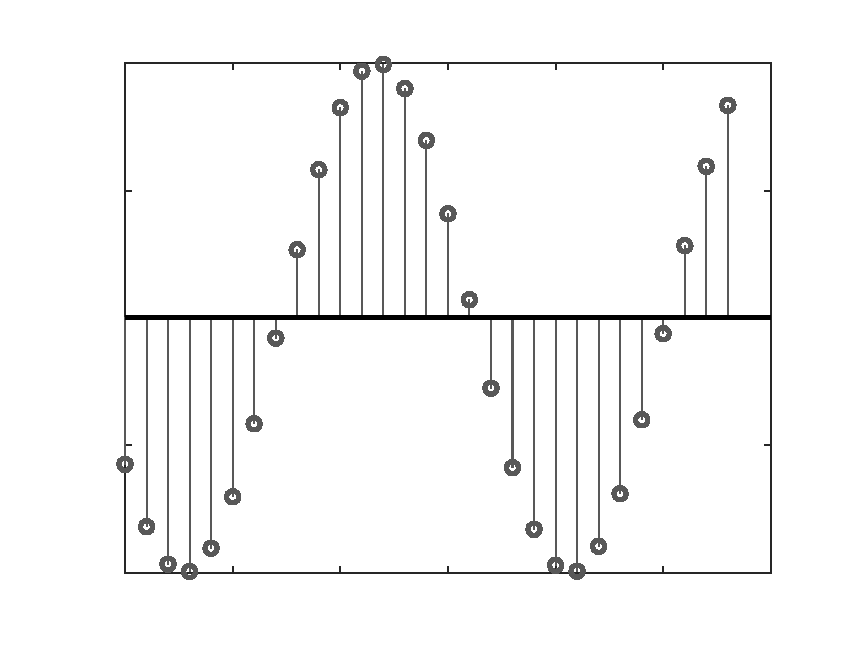
\includegraphics[scale=1]{octaves/stem-plot-inc}
\end{picture}%
\begin{picture}(400,300)(0,0)
\fontsize{6}{0}\selectfont\put(52,27.8){\makebox(0,0)[t]{\textcolor[rgb]{0.15,0.15,0.15}{{-10}}}}
\fontsize{6}{0}\selectfont\put(103.667,27.8){\makebox(0,0)[t]{\textcolor[rgb]{0.15,0.15,0.15}{{-5}}}}
\fontsize{6}{0}\selectfont\put(155.333,27.8){\makebox(0,0)[t]{\textcolor[rgb]{0.15,0.15,0.15}{{0}}}}
\fontsize{6}{0}\selectfont\put(207,27.8){\makebox(0,0)[t]{\textcolor[rgb]{0.15,0.15,0.15}{{5}}}}
\fontsize{6}{0}\selectfont\put(258.667,27.8){\makebox(0,0)[t]{\textcolor[rgb]{0.15,0.15,0.15}{{10}}}}
\fontsize{6}{0}\selectfont\put(310.333,27.8){\makebox(0,0)[t]{\textcolor[rgb]{0.15,0.15,0.15}{{15}}}}
\fontsize{6}{0}\selectfont\put(362,27.8){\makebox(0,0)[t]{\textcolor[rgb]{0.15,0.15,0.15}{{20}}}}
\fontsize{6}{0}\selectfont\put(48.5263,33){\makebox(0,0)[r]{\textcolor[rgb]{0.15,0.15,0.15}{{-1}}}}
\fontsize{6}{0}\selectfont\put(48.5263,94.125){\makebox(0,0)[r]{\textcolor[rgb]{0.15,0.15,0.15}{{-0.5}}}}
\fontsize{6}{0}\selectfont\put(48.5263,155.25){\makebox(0,0)[r]{\textcolor[rgb]{0.15,0.15,0.15}{{0}}}}
\fontsize{6}{0}\selectfont\put(48.5263,216.375){\makebox(0,0)[r]{\textcolor[rgb]{0.15,0.15,0.15}{{0.5}}}}
\fontsize{6}{0}\selectfont\put(48.5263,277.5){\makebox(0,0)[r]{\textcolor[rgb]{0.15,0.15,0.15}{{1}}}}
\fontsize{7}{0}\selectfont\put(207,287.5){\makebox(0,0)[b]{\textcolor[rgb]{0,0,0}{{A stem plot of a sinusoidal sequence}}}}
\end{picture}

}\caption{\emph{Stem plot} of a sinusoidal function. In particular, a stem plot of \texttt{cos(.35*x - .6)} has been performed with the help of the \texttt{octave} CLI. Pre-built binaries of the program are available at their website \texttt{https://octave.org/}.}\label{oct:stemPlot}
\end{center}
\end{figure}

Two kinds of digital signal representation exist. The first type is the common
digital signal where each sample is represented with a dot and a straight
line, while a \emph{boxedcar} signal will see each sample represented as a
straight line, in a similar fashion to the interpolation.

\subsubsection{Complex signals}

A signal can be either real or complex valued. A \emph{real se\-quen\-ce} comprises
only real samples such that $x[i] \in \R, \forall i \in \Z$ while a
\emph{complex se\-quen\-ce} has at least one complex sample $x[k] \in \C$. Complex
se\-quen\-ces may be seen as the result of the sum of two, distinct, real
se\-quen\-ces. In particular, by writing \[\{x[n]\} = \{x_{re}[n]\} +
j\{x_{im}[n]\}\] two different se\-quen\-ces, one for real part and the other one
for the imaginary part, are summed to form a single complex signal. It's easy
to understand that a real valued signal can still be written as a complex
signal, provided that $x_{im}[n] \equiv 0, \forall n$.

A complex signal's short, alternative notation is \[\{x[n]\} = \{A[n]e^{-j\cdot
f_t n}\},\] where the imaginary and real part are intrinsic in the exponential
representation and can thus be obtained by decomposing it into a sine and a
cosine addenda.

\subsubsection{Length of a signal}

A signal can either be of \emph{finite} or \emph{infinite}-length. In the first case defined values for the se\-quen\-ce lay only in an interval $N_1 \leq n \leq N_2$, with $N_1 \leq N_2$ and both $-\infty < |N_1| \leq |N_2| < \infty$. The overall \emph{length} or \emph{duration} of the se\-quen\-ce will be $N = N_2 - N_1 + 1$. In the second case a se\-quen\-ce is defined for every value of $n \in \Z$, after a certain $n_0$. For instance, $\{\cos{f_0 n}\}$ is an infinite-length se\-quen\-ce, because the signal ``never ends'', as there is no $n_1$ after which or before which the signal is null. Other infinite-length signals are any signal defined for all values after an $n_0 \in \Z$.

In practice, no signal really has infinite length, but it could be useful to still think of signals as such to make them more mathematically treatable.

\subsubsection{Zero-padding}

A signal may see its length varied by arbitrary operations. A very common operation in that regard, is to increase the length of a signal by appending or prepending $0$s to the signal, with a process called \textbf{zero-padding}. This usually involves a finite-length signal becoming an infinite-length signal by applying an infinitely long list of $0$s on both sides of the original signal; it is not uncommon, however, to apply the zero-padding technique to only one side of the signal. Another way to handle zero-padding is to simply add a finite---yet necessary---number of $0$s depending on the duty to perform.

\subsubsection{Causality}

A se\-quen\-ce is said to be \emph{right-sided} if it has zero-valued samples for each $n < N_1$. A special case of right-sided se\-quen\-ce is when $N_1 \geq 0$, the case of a \textbf{causal} signal.

Vice-versa, a se\-quen\-ce is said to be \emph{left-sided} if it has zero-valued samples for each $n > N_2$. The same way, when a left-sided se\-quen\-ce has $N_2 \leq 0$, we are in the case of an \textbf{anti-causal} signal.

Basically, causal signals are all signals that ``are relevant only \emph{after} a certain time $N_1$'', and anti-causal signals are all signals that ``are relevant \emph{before} a given time $N_2$''.

\subsubsection{Strength of a signal and signal comparison}

An important concept is the \textbf{strength} of a signal, also called \emph{size} of a signal. The strength of a signal is the $\mathcal{L}_p$-norm of the se\-quen\-ce,
\[
||x||_p = \left(\sum_{i=N_1}^{N_2} |x[n]|^p\right)^{\frac{1}{p}},
\]
where $p \in \N \setminus \{0\}$ is a positive integer, which is different from zero. Typically, one has $p=1,2,\infty$, with $p=2$ being the \emph{root mean squares} apart from a scaling factor---RMS is the square root of the \textbf{mean} of the squares, there's an additional $\frac{1}{\sqrt{n}}$ factor. The other two cases are $p=1$ corresponding to the \emph{mean absolute value} of the signal---except from a constant factor---and $p=\infty$ where the strength of the signal would be the \emph{absolute peak value} of the signal.

From the concept of signal strength the concept of \emph{relative error} immediately follows. In particular, let $\{y[n]\}, 0 \leq n \leq N - 1$ be an approximation of the signal $\{x[n]\}, 0 \leq n \leq N - 1$. In this case, one calls relative error the quantity
\begin{equation}\label{eqn:RelativeError}
	E_{rel} = \left(\frac{\sum_{n=0}^{N-1} |y[n] - x[n]|^2}{\sum_{n=0}^{N-1} |x[n]|^2}\right)^\frac{1}{2},
\end{equation}
which is the ratio of the $\mathcal L_2$-norm of the difference signal and the $\mathcal L_2$-norm of the signal $\{x[n]\}$. Everything is square-rooted.

The numerator of such quantity can be considered as the error between se\-quen\-ces $x$ and $y$, while the denominator is the $2$-strength of a non-approximated se\-quen\-ce.

\subsection{Operations on se\-quen\-ces}\label{sec:operationsOnSequences}

se\-quen\-ces may be subject to \emph{operations}. In particular, operations can be described by directed graphs in which there is an input se\-quen\-ce and an output se\-quen\-ce resulting from the operation. Of course, there may be more than one inputs or outputs.

    \begin{figure}[ht]
\begin{center}
\begin{tikzpicture}

    \node                 (input)                                 {$\{x[n]\}$};
    \node[squarednode]    (operation)     [right=of input]        {Operation};
    \node                 (output)        [right=of operation]    {$\{y[n]\}$};

    \draw[->] (input.east) -- (operation.west);
    \draw[->] (operation.east) -- (output.west);
\end{tikzpicture}\caption{The general scheme for elementary operations.}\label{tikz:operation-scheme}
\end{center}
\end{figure}

Basic signal operations are called \textbf{elementary operations}. The first
elementary operation is the \emph{modulation}, an operation in which a signal
$x$ is multiplied by another signal, say $w$, to produce an output signal $y$
such that $$y[n] = x[n]\cdot w[n].$$ A common application of the modulation is
the \emph{windowing} process, in which an infinite-length signal $x$ is
``windowed'' by a finite-length signal $w$, whose non-zero values are limited
to a finite interval and the non-zero values are all equal to $1$. In that
case, it would be like ``selecting'' the values of $x$ that lay in the $w$
window. Modulation is denoted with a cross inside a circle, as shown in Diagram~\ref{tikz:modulation-operation}.

\begin{figure}[ht]
\begin{center}
    \begin{tikzpicture}
    \node [](A){$x[n]$};
    \node [draw, fill=purple!15,circle,crossp, thick,minimum width=0.5 cm](B) at (1,0){};
    \node [](C) at(2,0){$y[n]$};
    \node [](D) at(1,-1){$w[n]$};
    \draw[->] (A) -- (B);
    \draw[->] (B) -- (C);
    \draw[->] (D) -- (B);
\end{tikzpicture}\caption{Notation for the modulation (product) operation.}\label{tikz:modulation-operation}
\end{center}
\end{figure}

Other elementary operations are the \emph{multiplication} operation and the \emph{addition} operation. The multiplier is denoted by a triangle---an opamp-like symbol is adopted---while the addition is a plus symbol inside a circle. Diagrams~\ref{tikz:multiplication-operation} and~\ref{tikz:addition-operation} summarize the overall notation. This time, multiplication is not performed between entire signals, but instead a constant $A$ multiplies a signal $x$, such that $$y[n] = A \cdot x[n].$$ The addition is performed between two distinct signals, hence $$z[n] = x[n] + y[n].$$

\begin{figure}[ht]
\begin{center}
    \begin{tikzpicture}
    \node [](A){$x[n]$};
    \node [draw, fill=red!10,isosceles triangle,thick,minimum width=.4 cm](B) at (1.5,0){$A$};
    \node [](C) at(3,0){$y[n]$};
    \draw[->] (A) -- (B);
    \draw[->] (B) -- (C);
\end{tikzpicture}\caption{Notation for the multiplication (product for a constant) operation.}\label{tikz:multiplication-operation}
\end{center}
\end{figure}

\begin{figure}[ht]
\begin{center}
\begin{tikzpicture}
    \node [](A) at (0,0){$x[n]$};
    \node [draw, fill=green!15,circle,plus,thick,minimum width=.5 cm](B) at (1,0){};
    \node [](C) at(2,0){$z[n]$};
    \node [](D) at(1,-1){$y[n]$};
    \draw[->] (A) -- (B);
    \draw[->] (B) -- (C);
    \draw[->] (D) -- (B);
\end{tikzpicture}\caption{Notation for the addition (sum) operation.}\label{tikz:addition-operation}
\end{center}
\end{figure}

Much relevant elementary operations are, indeed, the \emph{time delay} and
\emph{time advance}. A signal that is time-delayed is a signal which is a copy
of the original signal, but translated in time (delayed in this case).
Vice-versa, in the case of time advance, the signal copy of the original will be
anticipated. In the first case, the adopted symbol is $z^{-1}$, while for the
anticipation it is $z$. Hence, $y[n] = x[n - 1]$ and $y[n] = x[x + 1]$.

\begin{figure}[ht]
\begin{center}
    \begin{tikzpicture}
    \node [](A){$x[n]$};
    \node [draw, fill=red!10,boxfilter](B) at (1.5,0){$z^{-1}$};
    \node [](C) at(3,0){$x[n-1]$};
    \draw[->] (A) -- (B);
    \draw[->] (B) -- (C);
\end{tikzpicture}\caption{Notation for the time delaying operation.}\label{tikz:delaying-operation}
\end{center}
\end{figure}

\begin{figure}[ht]
\begin{center}
    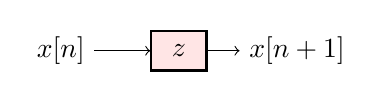
\begin{tikzpicture}
    \node [](A){$x[n]$};
    \node [draw, fill=red!10,rectangle,thick,minimum width=.7 cm, minimum height=.5cm](B) at (1.5,0){$z$};
    \node [](C) at(3,0){$x[n+1]$};
    \draw[->] (A) -- (B);
    \draw[->] (B) -- (C);
\end{tikzpicture}\caption{Notation for the time advance operation.}\label{tikz:advance-operation}
\end{center}
\end{figure}

An interesting operation is the \emph{time reversal} or \emph{folding}. The folding operation inverts the time axis of a signal, that means $y[n] = x[-n]$. Time reversal does not have any explicit symbol, since it requires a complete reflection of a signal from its origin point.

Yet another common `operation' is the \emph{branching} operation, in which a signal $w$ is simply the copy of the input signal, as well as the $y$ signal (a single input is copied into two outputs). Branching is shown in Diagram~\ref{tikz:branchingOperation}.
\begin{figure}[ht]
\begin{center}
    \begin{tikzpicture}
    \node [](A){$x[n]$};
    \node [draw, fill=black!100,inner sep=1pt,circle,label=above:{b}](B) at (1.5,0){};
    \node [](C) at(3,0){$x[n]$};
    \node [](D) at(1.5,-1.5){$x[n]$};
    \draw[->] (A) -- (B) -- (C);
    \draw[->] (B) -- (D);
\end{tikzpicture}\caption{Notation for the branching (signal splitting) operation. The $b$ node allows splitting of the signal into two---equal---branches where $x$ is routed.}\label{tikz:branchingOperation}
\end{center}
\end{figure}

In order to apply most of the above operations, two signals should possess the same length---in those cases where this does not occur, a \emph{zero-padding} is required. For instance, to perform addition on two signals, the two signals must share the same length, therefore it is mandatory to at least perform a zero-padding on the shortest of the signals. Infinitely long signals can always be summed together.

Multiple elementary operations can be combined as well, by building a directed graph in which the signals are subject to multiple eventual operations, in the order determined by the particular graph. Usually, multiple operations should be necessary and are therefore applied in special manners to obtain the desired result.

\section{Ensemble Averaging}

A very powerful operation to apply to a signal is the \textbf{ensemble averaging}. Ensemble averaging is the operation of performing an average of a signal when multiple, independent measures are available. The goal of the ensemble averaging is to enhance the quality of a signal with respect to a noise which affects it. In other words, the result is expected to suffer less from noise than the original signal.

Suppose $i$-th measured signal $x_i$ has two components $x_i = s + d_i$, the
first one relative to an original signal $s$ and the noise component $d_i$, which
varies according to the measurement. The ensamble average of the $K$ measurements is the signal $x_{avg}$ such that
\begin{equation}\label{eqn:EnsambleAveraging}
	x_{avg} = \frac{1}{K}\sum_{i=1}^{K} s + d_i = s + \frac{1}{K}\sum_{i=1}^{K}d_i,
\end{equation}
which tends to the original signal $s$ as the number of signals $K \rightarrow \infty$ approaches infinity. The benefit of the ensemble averaging lies in the fact that the variance of the white noise $d_i$ is reduced by a factor of $K$, leading to a reasonable replica of the original signal $s$. An example of application of ensemble averaging is shown in Figure~\ref{oct:ensembleAveraging}.

\begin{figure*}[ht]
\begin{center}
\scalebox{0.32}{
% Title: gl2ps_renderer figure
% Creator: GL2PS 1.4.2, (C) 1999-2020 C. Geuzaine
% For: Octave
% CreationDate: Wed Oct 19 09:01:13 2022
\setlength{\unitlength}{1pt}
\begin{picture}(0,0)
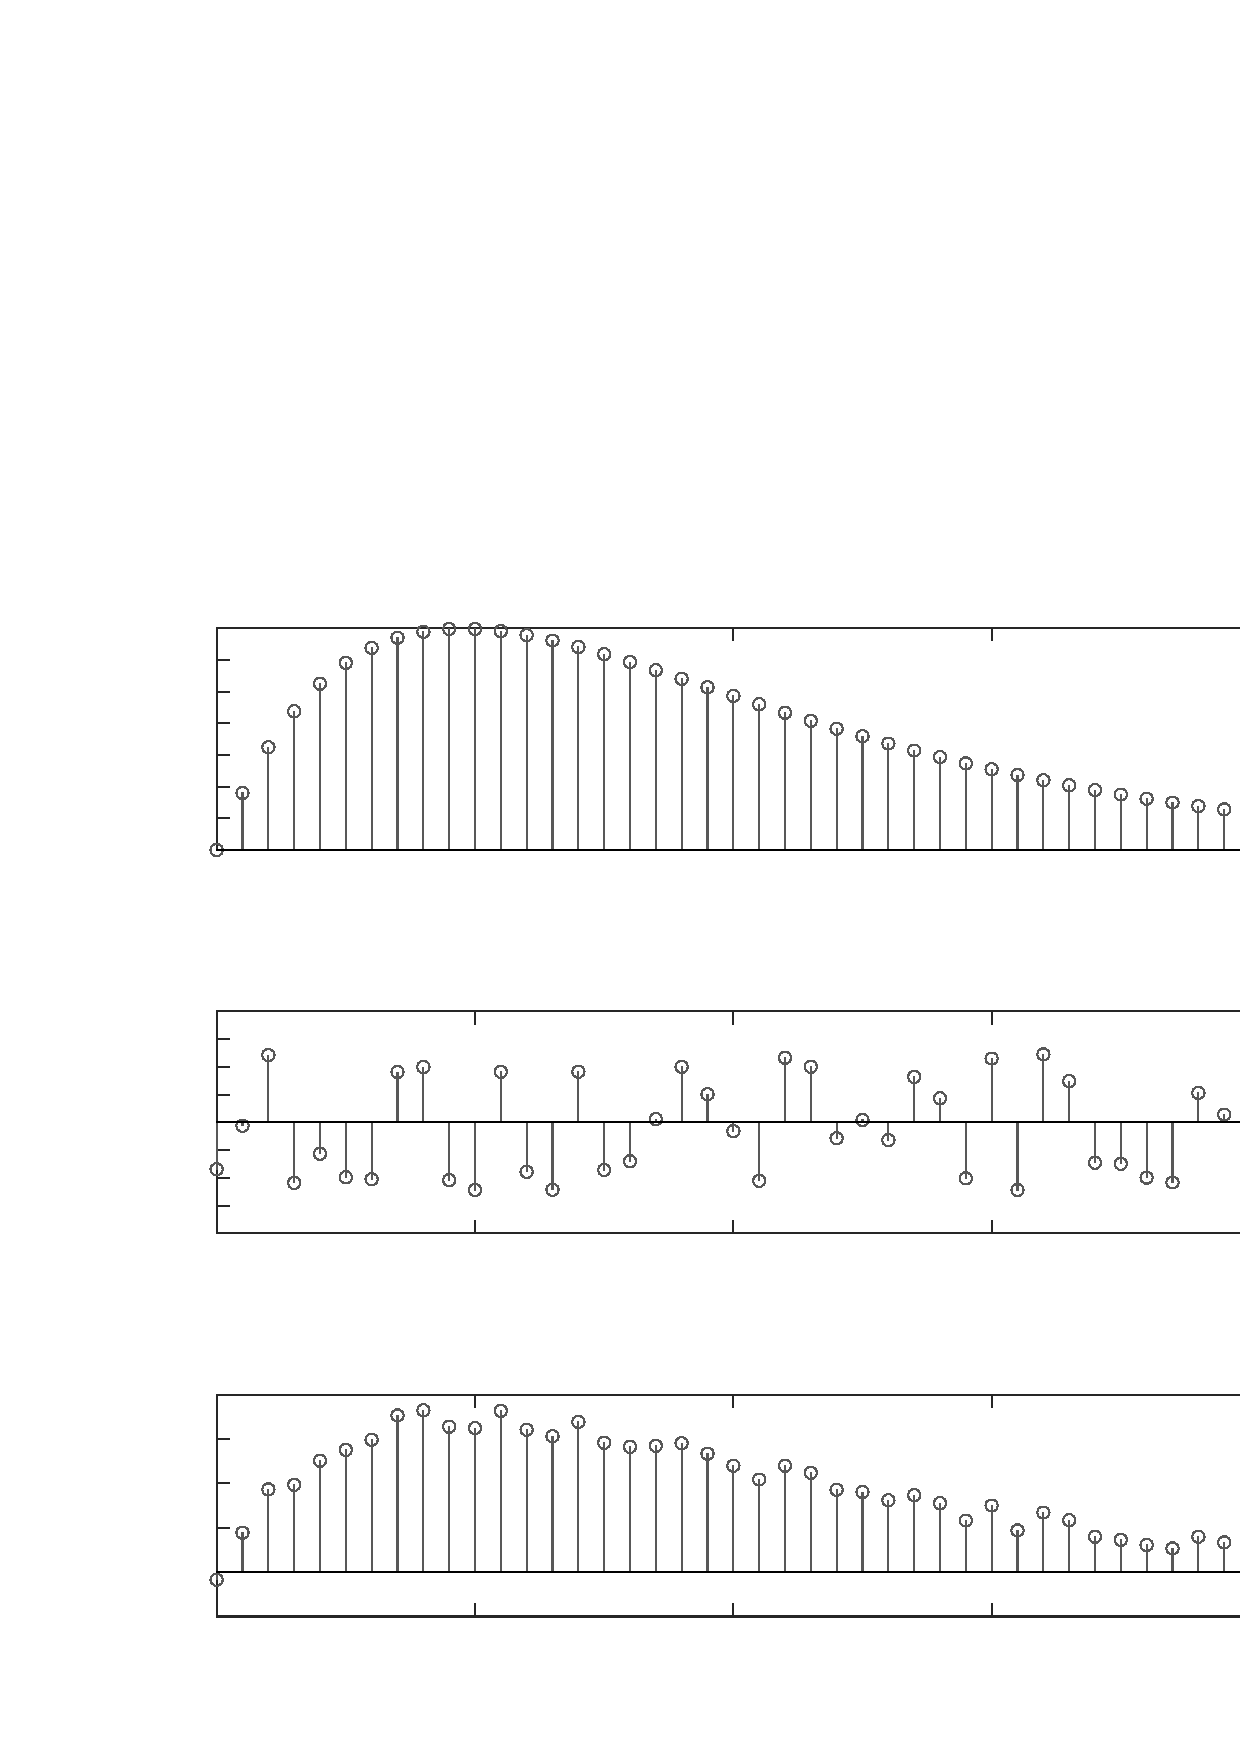
\includegraphics[scale=1]{octaves/ensembleAveraging-inc}
\end{picture}%
\begin{picture}(800,600)(0,0)
\fontsize{13}{0}\selectfont\put(104,423.523){\makebox(0,0)[t]{\textcolor[rgb]{0.15,0.15,0.15}{{0}}}}
\fontsize{13}{0}\selectfont\put(228,423.523){\makebox(0,0)[t]{\textcolor[rgb]{0.15,0.15,0.15}{{10}}}}
\fontsize{13}{0}\selectfont\put(352,423.523){\makebox(0,0)[t]{\textcolor[rgb]{0.15,0.15,0.15}{{20}}}}
\fontsize{13}{0}\selectfont\put(476,423.523){\makebox(0,0)[t]{\textcolor[rgb]{0.15,0.15,0.15}{{30}}}}
\fontsize{13}{0}\selectfont\put(600,423.523){\makebox(0,0)[t]{\textcolor[rgb]{0.15,0.15,0.15}{{40}}}}
\fontsize{13}{0}\selectfont\put(724,423.523){\makebox(0,0)[t]{\textcolor[rgb]{0.15,0.15,0.15}{{50}}}}
\fontsize{13}{0}\selectfont\put(97.0525,433.898){\makebox(0,0)[r]{\textcolor[rgb]{0.15,0.15,0.15}{{0}}}}
\fontsize{13}{0}\selectfont\put(97.0525,449.116){\makebox(0,0)[r]{\textcolor[rgb]{0.15,0.15,0.15}{{1}}}}
\fontsize{13}{0}\selectfont\put(97.0525,464.334){\makebox(0,0)[r]{\textcolor[rgb]{0.15,0.15,0.15}{{2}}}}
\fontsize{13}{0}\selectfont\put(97.0525,479.552){\makebox(0,0)[r]{\textcolor[rgb]{0.15,0.15,0.15}{{3}}}}
\fontsize{13}{0}\selectfont\put(97.0525,494.77){\makebox(0,0)[r]{\textcolor[rgb]{0.15,0.15,0.15}{{4}}}}
\fontsize{13}{0}\selectfont\put(97.0525,509.988){\makebox(0,0)[r]{\textcolor[rgb]{0.15,0.15,0.15}{{5}}}}
\fontsize{13}{0}\selectfont\put(97.0525,525.206){\makebox(0,0)[r]{\textcolor[rgb]{0.15,0.15,0.15}{{6}}}}
\fontsize{13}{0}\selectfont\put(97.0525,540.424){\makebox(0,0)[r]{\textcolor[rgb]{0.15,0.15,0.15}{{7}}}}
\fontsize{15}{0}\selectfont\put(414,550.424){\makebox(0,0)[b]{\textcolor[rgb]{0,0,0}{{Original uncorrupted sequence}}}}
\fontsize{15}{0}\selectfont\put(84.0526,487.161){\rotatebox{90}{\makebox(0,0)[b]{\textcolor[rgb]{0.15,0.15,0.15}{{Amplitude}}}}}
\fontsize{15}{0}\selectfont\put(414,407.523){\makebox(0,0)[t]{\textcolor[rgb]{0.15,0.15,0.15}{{Time index n}}}}
\fontsize{13}{0}\selectfont\put(104,239.574){\makebox(0,0)[t]{\textcolor[rgb]{0.15,0.15,0.15}{{0}}}}
\fontsize{13}{0}\selectfont\put(228,239.574){\makebox(0,0)[t]{\textcolor[rgb]{0.15,0.15,0.15}{{10}}}}
\fontsize{13}{0}\selectfont\put(352,239.574){\makebox(0,0)[t]{\textcolor[rgb]{0.15,0.15,0.15}{{20}}}}
\fontsize{13}{0}\selectfont\put(476,239.574){\makebox(0,0)[t]{\textcolor[rgb]{0.15,0.15,0.15}{{30}}}}
\fontsize{13}{0}\selectfont\put(600,239.574){\makebox(0,0)[t]{\textcolor[rgb]{0.15,0.15,0.15}{{40}}}}
\fontsize{13}{0}\selectfont\put(724,239.574){\makebox(0,0)[t]{\textcolor[rgb]{0.15,0.15,0.15}{{50}}}}
\fontsize{13}{0}\selectfont\put(97.0525,249.949){\makebox(0,0)[r]{\textcolor[rgb]{0.15,0.15,0.15}{{-0.8}}}}
\fontsize{13}{0}\selectfont\put(97.0525,263.265){\makebox(0,0)[r]{\textcolor[rgb]{0.15,0.15,0.15}{{-0.6}}}}
\fontsize{13}{0}\selectfont\put(97.0525,276.58){\makebox(0,0)[r]{\textcolor[rgb]{0.15,0.15,0.15}{{-0.4}}}}
\fontsize{13}{0}\selectfont\put(97.0525,289.896){\makebox(0,0)[r]{\textcolor[rgb]{0.15,0.15,0.15}{{-0.2}}}}
\fontsize{13}{0}\selectfont\put(97.0525,303.212){\makebox(0,0)[r]{\textcolor[rgb]{0.15,0.15,0.15}{{0}}}}
\fontsize{13}{0}\selectfont\put(97.0525,316.527){\makebox(0,0)[r]{\textcolor[rgb]{0.15,0.15,0.15}{{0.2}}}}
\fontsize{13}{0}\selectfont\put(97.0525,329.843){\makebox(0,0)[r]{\textcolor[rgb]{0.15,0.15,0.15}{{0.4}}}}
\fontsize{13}{0}\selectfont\put(97.0525,343.159){\makebox(0,0)[r]{\textcolor[rgb]{0.15,0.15,0.15}{{0.6}}}}
\fontsize{13}{0}\selectfont\put(97.0525,356.475){\makebox(0,0)[r]{\textcolor[rgb]{0.15,0.15,0.15}{{0.8}}}}
\fontsize{15}{0}\selectfont\put(414,366.475){\makebox(0,0)[b]{\textcolor[rgb]{0,0,0}{{Noise}}}}
\fontsize{15}{0}\selectfont\put(68.0525,303.212){\rotatebox{90}{\makebox(0,0)[b]{\textcolor[rgb]{0.15,0.15,0.15}{{Amplitude}}}}}
\fontsize{15}{0}\selectfont\put(414,223.574){\makebox(0,0)[t]{\textcolor[rgb]{0.15,0.15,0.15}{{Time index n}}}}
\fontsize{13}{0}\selectfont\put(104,55.625){\makebox(0,0)[t]{\textcolor[rgb]{0.15,0.15,0.15}{{0}}}}
\fontsize{13}{0}\selectfont\put(228,55.625){\makebox(0,0)[t]{\textcolor[rgb]{0.15,0.15,0.15}{{10}}}}
\fontsize{13}{0}\selectfont\put(352,55.625){\makebox(0,0)[t]{\textcolor[rgb]{0.15,0.15,0.15}{{20}}}}
\fontsize{13}{0}\selectfont\put(476,55.625){\makebox(0,0)[t]{\textcolor[rgb]{0.15,0.15,0.15}{{30}}}}
\fontsize{13}{0}\selectfont\put(600,55.625){\makebox(0,0)[t]{\textcolor[rgb]{0.15,0.15,0.15}{{40}}}}
\fontsize{13}{0}\selectfont\put(724,55.625){\makebox(0,0)[t]{\textcolor[rgb]{0.15,0.15,0.15}{{50}}}}
\fontsize{13}{0}\selectfont\put(97.0525,66){\makebox(0,0)[r]{\textcolor[rgb]{0.15,0.15,0.15}{{-2}}}}
\fontsize{13}{0}\selectfont\put(97.0525,87.3051){\makebox(0,0)[r]{\textcolor[rgb]{0.15,0.15,0.15}{{0}}}}
\fontsize{13}{0}\selectfont\put(97.0525,108.61){\makebox(0,0)[r]{\textcolor[rgb]{0.15,0.15,0.15}{{2}}}}
\fontsize{13}{0}\selectfont\put(97.0525,129.915){\makebox(0,0)[r]{\textcolor[rgb]{0.15,0.15,0.15}{{4}}}}
\fontsize{13}{0}\selectfont\put(97.0525,151.22){\makebox(0,0)[r]{\textcolor[rgb]{0.15,0.15,0.15}{{6}}}}
\fontsize{13}{0}\selectfont\put(97.0525,172.525){\makebox(0,0)[r]{\textcolor[rgb]{0.15,0.15,0.15}{{8}}}}
\fontsize{15}{0}\selectfont\put(414,182.525){\makebox(0,0)[b]{\textcolor[rgb]{0,0,0}{{Corrupted sequence}}}}
\fontsize{15}{0}\selectfont\put(79.0526,119.263){\rotatebox{90}{\makebox(0,0)[b]{\textcolor[rgb]{0.15,0.15,0.15}{{Amplitude}}}}}
\fontsize{15}{0}\selectfont\put(414,39.6249){\makebox(0,0)[t]{\textcolor[rgb]{0.15,0.15,0.15}{{Time index n}}}}
\end{picture}

% Title: gl2ps_renderer figure
% Creator: GL2PS 1.4.2, (C) 1999-2020 C. Geuzaine
% For: Octave
% CreationDate: Wed Oct 19 09:02:39 2022
\setlength{\unitlength}{1pt}
\begin{picture}(0,0)
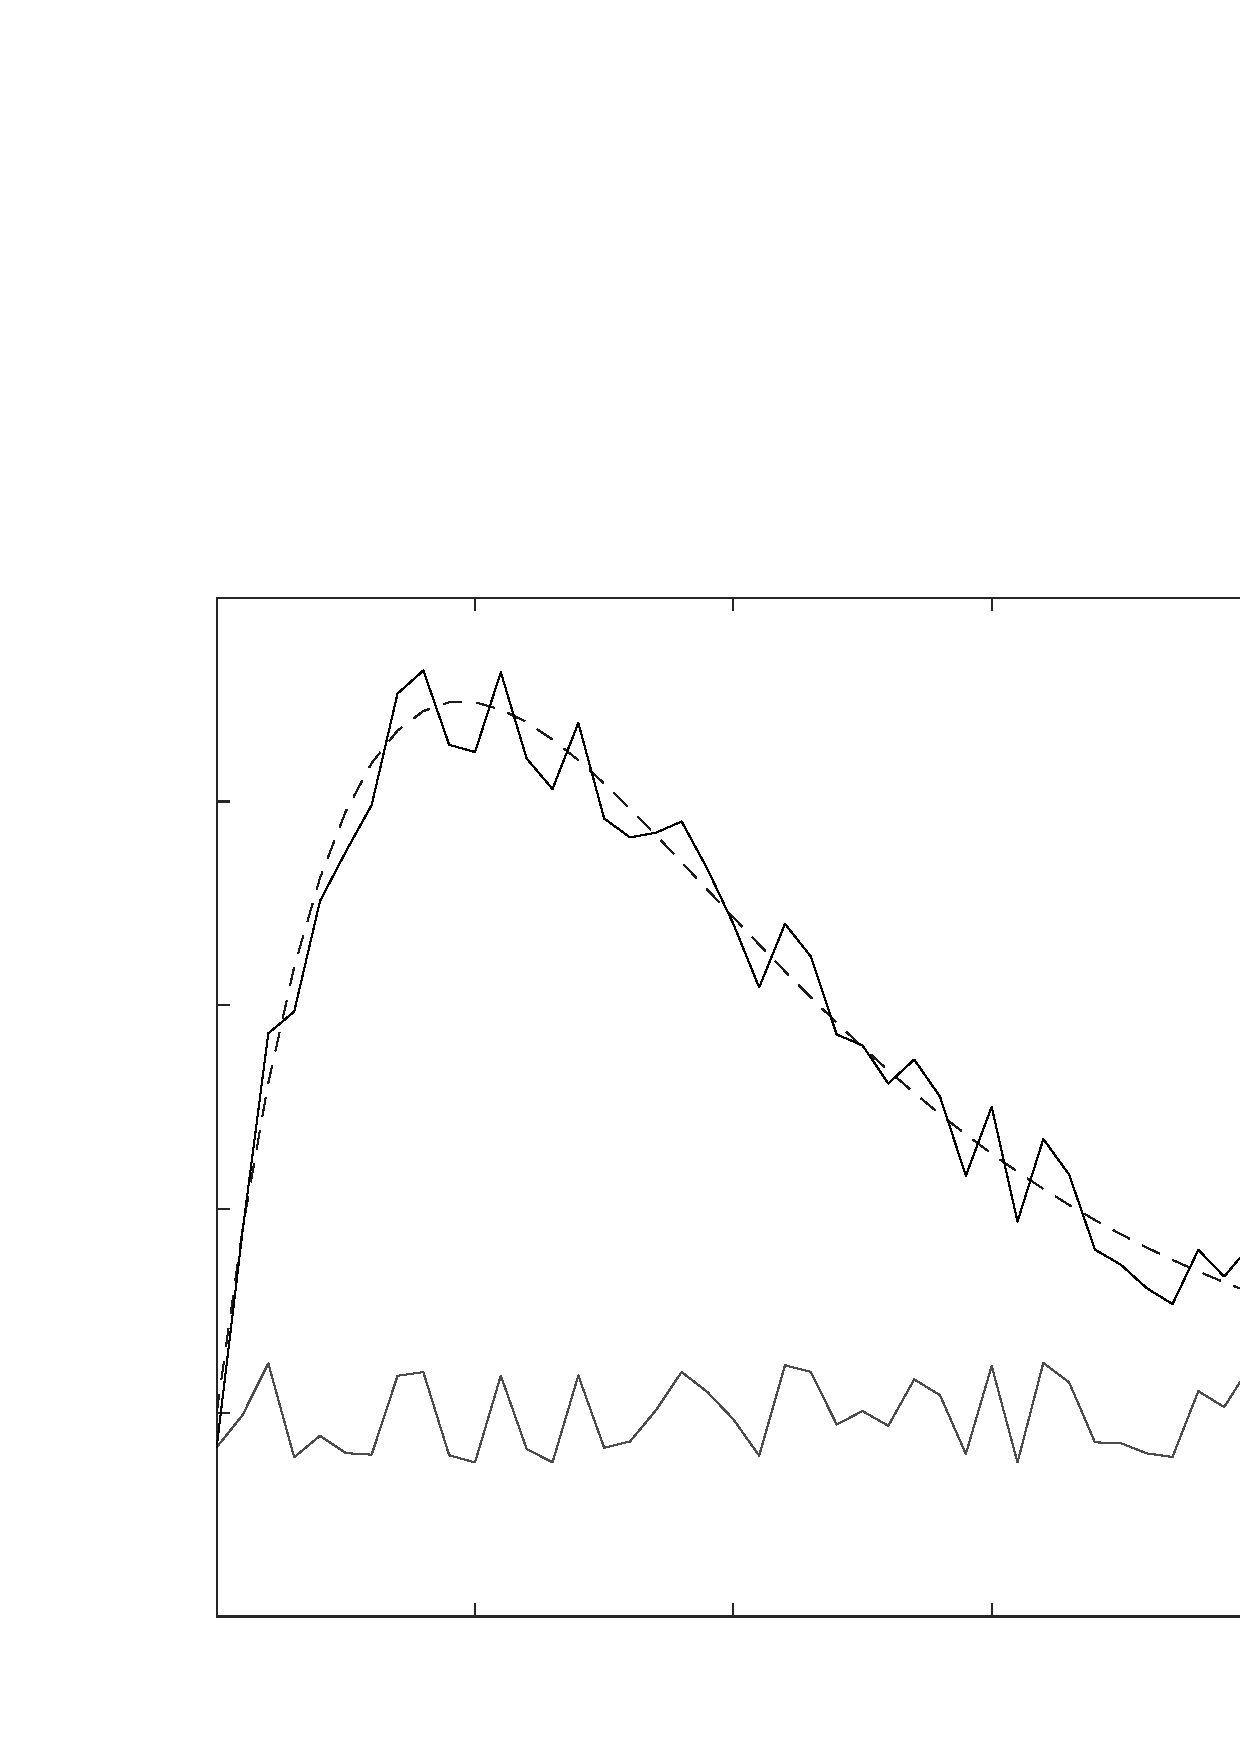
\includegraphics[scale=1]{octaves/ensembleAveragingTwo-inc}
\end{picture}%
\begin{picture}(800,600)(0,0)
\fontsize{13}{0}\selectfont\put(104,55.5788){\makebox(0,0)[t]{\textcolor[rgb]{0.15,0.15,0.15}{{0}}}}
\fontsize{13}{0}\selectfont\put(228,55.5788){\makebox(0,0)[t]{\textcolor[rgb]{0.15,0.15,0.15}{{10}}}}
\fontsize{13}{0}\selectfont\put(352,55.5788){\makebox(0,0)[t]{\textcolor[rgb]{0.15,0.15,0.15}{{20}}}}
\fontsize{13}{0}\selectfont\put(476,55.5788){\makebox(0,0)[t]{\textcolor[rgb]{0.15,0.15,0.15}{{30}}}}
\fontsize{13}{0}\selectfont\put(600,55.5788){\makebox(0,0)[t]{\textcolor[rgb]{0.15,0.15,0.15}{{40}}}}
\fontsize{13}{0}\selectfont\put(724,55.5788){\makebox(0,0)[t]{\textcolor[rgb]{0.15,0.15,0.15}{{50}}}}
\fontsize{13}{0}\selectfont\put(97.0525,66){\makebox(0,0)[r]{\textcolor[rgb]{0.15,0.15,0.15}{{-2}}}}
\fontsize{13}{0}\selectfont\put(97.0525,163.8){\makebox(0,0)[r]{\textcolor[rgb]{0.15,0.15,0.15}{{0}}}}
\fontsize{13}{0}\selectfont\put(97.0525,261.6){\makebox(0,0)[r]{\textcolor[rgb]{0.15,0.15,0.15}{{2}}}}
\fontsize{13}{0}\selectfont\put(97.0525,359.4){\makebox(0,0)[r]{\textcolor[rgb]{0.15,0.15,0.15}{{4}}}}
\fontsize{13}{0}\selectfont\put(97.0525,457.2){\makebox(0,0)[r]{\textcolor[rgb]{0.15,0.15,0.15}{{6}}}}
\fontsize{13}{0}\selectfont\put(97.0525,555){\makebox(0,0)[r]{\textcolor[rgb]{0.15,0.15,0.15}{{8}}}}
\fontsize{15}{0}\selectfont\put(414,39.5788){\makebox(0,0)[t]{\textcolor[rgb]{0.15,0.15,0.15}{{Time index n}}}}
\fontsize{15}{0}\selectfont\put(79.0526,310.5){\rotatebox{90}{\makebox(0,0)[b]{\textcolor[rgb]{0.15,0.15,0.15}{{Amplitude}}}}}
\fontsize{12}{0}\selectfont\put(693.005,536.005){\makebox(0,0)[l]{\textcolor[rgb]{0,0,0}{{x[n]}}}}
\fontsize{12}{0}\selectfont\put(693.005,518.007){\makebox(0,0)[l]{\textcolor[rgb]{0,0,0}{{y[n]}}}}
\end{picture}

}\caption{The ensemble averaging. On the left, the original uncorrupted sequence $s[n]$, the noise $d[n]$ and the corrupted sequence $x[n]$. On the right, the dashed line represents the sequence $y[n]$, a ``recovered'' version of the original sequence $s[n]$. Recovering has been performed by means of the ensemble averaging process.}\label{oct:ensembleAveraging}
\end{center}
\end{figure*}

\section{Sample Rate Alteration}

The operation of alterating the sample rate $F_S$ is much important. Generally, it is adopted to obtain a new signal $x'$ from a signal $x$, but with a different sample rate $F'_S$. The new sample rate can either be high\-er or lower than the original signal, so that a \emph{sampling rate alteration ratio} can be defined,
\begin{equation}\label{eqn:SamplingRateAlterationRatio}
	R_S = \frac{F'_S}{F_S}.
\end{equation}

The ratio in equation \ref{eqn:SamplingRateAlterationRatio} can either be greater or lower than $1$, and determines the nature of the sample rate alteration. In particolar, in the case of $R_S > 1$ one performs the \textbf{interpolation} operation, while in the opposite case of $R_S < 1$ one gets the \textbf{decimation} operation.

Two operations are imperative for, respectively, interpolation and decimation: the \emph{up-sampling} and the \emph{down-sam\-pling} operations. To be specific, in order to perform interpolation a \emph{further} operation is needed other than up-sampling.

\subsubsection{Up-Sampling}

The up-sampling operation by an integer factor $L > 1$ involves the addition of
$L-1$ zero-valued samples inserted between two consecutive samples of the
original signal:

\begin{equation}\label{eqn:UpSampling}
	x_u[n] =
	\left\{
		\begin{array}{ll}
			x[n/L] 	& n=0,\pm L, \pm 2L, \dots \\
			0 	& otherwise
		\end{array}
	\right.
\end{equation}

Up-sampling operation is denoted by a $\uparrow L$ block, as in Diagram~\ref{tikz:upsamplingOperation}. Upsampling is usually followed by \emph{interpolation}.

\begin{figure}[ht]
\begin{center}
    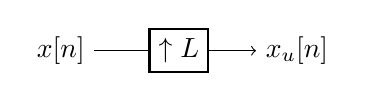
\begin{tikzpicture}
    \node [](A){$x[n]$};
    \node [draw,rectangle,thick](B) at (1.5,0){$\uparrow L$};
    \node [](C) at(3,0){$x_u[n]$};
    \draw[->] (A) -- (B) -- (C);
\end{tikzpicture}\caption{Notation for the up-sampling operation by a factor $L$.}\label{tikz:upsamplingOperation}
\end{center}
\end{figure}

\subsubsection{Down-Sampling}

The down-sampling operation by an integer factor $M > 1$ means that from the
original signal only one sample every $M$ is preserved. This way, $M-1$ consecutive
in between samples are removed from the signal, while a single one every $M$ samples is preserved,
\begin{equation}\label{eqn:DownSampling}
	x_d[n] = x[nM]
\end{equation}

Down-sampling operation is denoted by a $\downarrow M$ block, as in Figure~\ref{tikz:downsamplingOperation}.
\begin{figure}[ht]
\begin{center}
    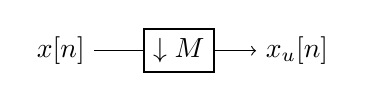
\begin{tikzpicture}
    \node [](A){$x[n]$};
    \node [draw,rectangle,thick](B) at (1.5,0){$\downarrow M$};
    \node [](C) at(3,0){$x_u[n]$};
    \draw[->] (A) -- (B) -- (C);
\end{tikzpicture}\caption{Notation for the down-sampling operation by a factor $M$.}\label{tikz:downsamplingOperation}
\end{center}
\end{figure}
The result of downsampling is a se\-quen\-ce in which some values are missing, those that are removed by the downsampling operation. A crucial risk of downsampling that we will tackle is the \textbf{aliasing} phenomenon.
\begin{figure*}[ht]
    \centering
    \scalebox{0.6}{
    % Title: gl2ps_renderer figure
% Creator: GL2PS 1.4.2, (C) 1999-2020 C. Geuzaine
% For: Octave
% CreationDate: Wed Oct 19 09:18:32 2022
\setlength{\unitlength}{1pt}
\begin{picture}(0,0)
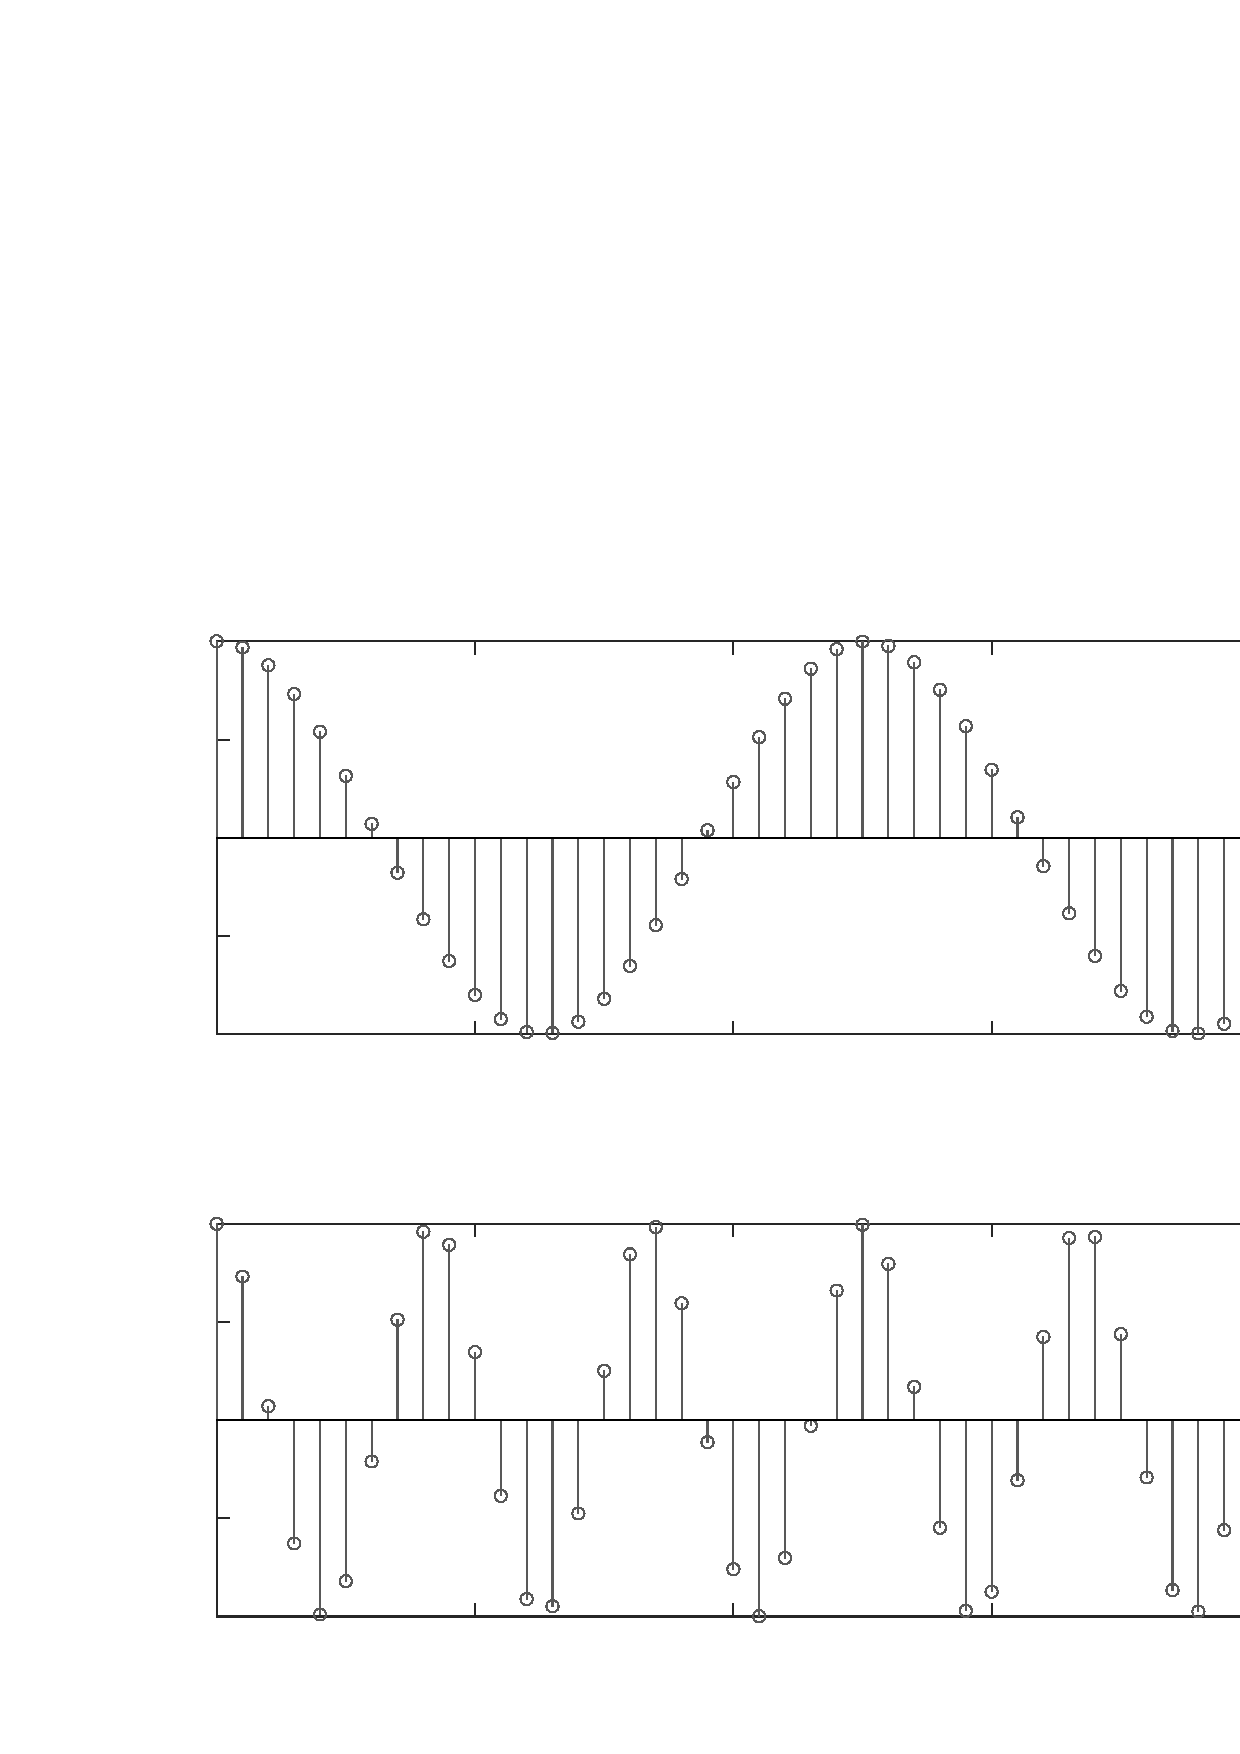
\includegraphics[scale=1]{octaves/downsamplingOperationEffect-inc}
\end{picture}%
\begin{picture}(800,600)(0,0)
\fontsize{13}{0}\selectfont\put(104,335.117){\makebox(0,0)[t]{\textcolor[rgb]{0.15,0.15,0.15}{{0}}}}
\fontsize{13}{0}\selectfont\put(228,335.117){\makebox(0,0)[t]{\textcolor[rgb]{0.15,0.15,0.15}{{10}}}}
\fontsize{13}{0}\selectfont\put(352,335.117){\makebox(0,0)[t]{\textcolor[rgb]{0.15,0.15,0.15}{{20}}}}
\fontsize{13}{0}\selectfont\put(476,335.117){\makebox(0,0)[t]{\textcolor[rgb]{0.15,0.15,0.15}{{30}}}}
\fontsize{13}{0}\selectfont\put(600,335.117){\makebox(0,0)[t]{\textcolor[rgb]{0.15,0.15,0.15}{{40}}}}
\fontsize{13}{0}\selectfont\put(724,335.117){\makebox(0,0)[t]{\textcolor[rgb]{0.15,0.15,0.15}{{50}}}}
\fontsize{13}{0}\selectfont\put(97.0525,345.566){\makebox(0,0)[r]{\textcolor[rgb]{0.15,0.15,0.15}{{-1}}}}
\fontsize{13}{0}\selectfont\put(97.0525,392.691){\makebox(0,0)[r]{\textcolor[rgb]{0.15,0.15,0.15}{{-0.5}}}}
\fontsize{13}{0}\selectfont\put(97.0525,439.816){\makebox(0,0)[r]{\textcolor[rgb]{0.15,0.15,0.15}{{0}}}}
\fontsize{13}{0}\selectfont\put(97.0525,486.941){\makebox(0,0)[r]{\textcolor[rgb]{0.15,0.15,0.15}{{0.5}}}}
\fontsize{13}{0}\selectfont\put(97.0525,534.066){\makebox(0,0)[r]{\textcolor[rgb]{0.15,0.15,0.15}{{1}}}}
\fontsize{15}{0}\selectfont\put(414,544.066){\makebox(0,0)[b]{\textcolor[rgb]{0,0,0}{{Original sequence}}}}
\fontsize{13}{0}\selectfont\put(104,55.6063){\makebox(0,0)[t]{\textcolor[rgb]{0.15,0.15,0.15}{{0}}}}
\fontsize{13}{0}\selectfont\put(228,55.6063){\makebox(0,0)[t]{\textcolor[rgb]{0.15,0.15,0.15}{{10}}}}
\fontsize{13}{0}\selectfont\put(352,55.6063){\makebox(0,0)[t]{\textcolor[rgb]{0.15,0.15,0.15}{{20}}}}
\fontsize{13}{0}\selectfont\put(476,55.6063){\makebox(0,0)[t]{\textcolor[rgb]{0.15,0.15,0.15}{{30}}}}
\fontsize{13}{0}\selectfont\put(600,55.6063){\makebox(0,0)[t]{\textcolor[rgb]{0.15,0.15,0.15}{{40}}}}
\fontsize{13}{0}\selectfont\put(724,55.6063){\makebox(0,0)[t]{\textcolor[rgb]{0.15,0.15,0.15}{{50}}}}
\fontsize{13}{0}\selectfont\put(97.0525,66){\makebox(0,0)[r]{\textcolor[rgb]{0.15,0.15,0.15}{{-1}}}}
\fontsize{13}{0}\selectfont\put(97.0525,113.125){\makebox(0,0)[r]{\textcolor[rgb]{0.15,0.15,0.15}{{-0.5}}}}
\fontsize{13}{0}\selectfont\put(97.0525,160.25){\makebox(0,0)[r]{\textcolor[rgb]{0.15,0.15,0.15}{{0}}}}
\fontsize{13}{0}\selectfont\put(97.0525,207.375){\makebox(0,0)[r]{\textcolor[rgb]{0.15,0.15,0.15}{{0.5}}}}
\fontsize{13}{0}\selectfont\put(97.0525,254.5){\makebox(0,0)[r]{\textcolor[rgb]{0.15,0.15,0.15}{{1}}}}
\fontsize{15}{0}\selectfont\put(414,264.5){\makebox(0,0)[b]{\textcolor[rgb]{0,0,0}{{Downsampled sequence by a factor of 3}}}}
\end{picture}

    }\caption{Example of down-sampling operation applied to a sinusoidal input se\-quen\-ce.}\label{oct:downsamplingOperationEffect}
\end{figure*}


\section{Classification of se\-quen\-ces}

There are several ways to classify a se\-quen\-ce.

The first one is by \textbf{symmetry}. A \emph{conjugate-symmetric} se\-quen\-ce is a se\-quen\-ce that satisfies the property \[x[n] = x^*[-n];\] If $x$ is real, then it is said to be an \emph{even se\-quen\-ce}. The \emph{conjugate antisymetric se\-quen\-ce}, on contrary, is such that \[x[n] = -x^*[-n],\] and if $x$ is real, then it is said to be an \emph{odd se\-quen\-ce}. Every se\-quen\-ce can be defined with the sum of its conjugate symmetric and antisimetric parts\footnote{In fact, $x_{cs} = \frac{1}{2}(x[n] + x^*[-n])$ and $x_{as} = \frac{1}{2}(x[n] - x^*[-n])$.}, that are two distinct signals \[x[n] = x_{cs}[n] + x_{ca}[n];\]

Another way is by \textbf{periodicity}: a se\-quen\-ce $\tilde{x}[n]$ is \emph{periodic with period} $N$ if it satisfies the property \[\tilde{x}[n] = \tilde{x}[n + kN]\] for some $N \in \Z$. Smallest $N$ value that satisfies such property is called \emph{fundamental period}. A se\-quen\-ce that does not satisfy this property is said to be \emph{aperiodic}. The sum of two periodic signals $x_a$ and $x_b$ of fundamental period---respectively---$N_a$ and $N_b$ is still a periodic se\-quen\-ce, having fundamental period $N_f$ of \[N_f = \frac{N_a N_b}{\mathrm{GCD}(N_a, N_b)} \geq \max{(N_a, N_b)},\] where $\mathrm{GCD}$ is the ``greatest common divisor'' operation;

One can also compute the \textbf{total energy} of a signal $x$, defined as the quantity
\begin{equation}\label{eqn:totalEnergy}
    \mathcal E_x = \sum_{n=-\infty}^{\infty} | x[n] |^2.
\end{equation}
A finite-length se\-quen\-ce will possess finite energy, but an infinite-length se\-quen\-ce might have finite or infinite energy depending on the nature of the signal. Among with the definition of energy, it comes the definition of \textbf{average power} of a signal, which is, specifically,
\begin{equation}\label{eqn:averagePower}
    P_x = \lim_{K \rightarrow \infty} \frac{1}{2K + 1} \sum_{n = -K}^K |x[n]|^2.
\end{equation}
The average power formula may depend on the nature of the signal. In particular,
\begin{itemize}
    \item regarding \emph{aperiodic} signals, the average power is
        \[ P_x = \lim_{K \rightarrow \infty} \frac{1}{2K + 1} \sum_{n = -K}^K |x[n]|^2, \]
    and---recalling the definition of total energy---can thus be rewritten as
    \[ P_x = \lim_{K \rightarrow \infty} \frac{1}{2K + 1} \mathcal E_{x,K}; \]
    \item regarding \emph{periodic} signals with period $N$, the average power is
        \[P_x = \frac{1}{N} \sum_{n = 0}^{N-1} |x[n]|^2,\] a quantity that is computed through a period and might be finite or infinite\footnote{To introduce some examples, consider a causal se\-quen\-ce defined by \[ x[n] = \left\{\begin{array}{lc}3(-1)^n, & n \geq 0\\ 0, & n < 0\end{array}\right. .\] se\-quen\-ce $x$ has infinite energy. The average power is given by \[P_x = \lim_{K\rightarrow \infty}\frac{1}{2K+1}\left(9\sum_{n=0}^K 1\right) = \lim_{K\rightarrow \infty}\frac{9(K+1)}{2K+1} = 4.5,\] a finite quantity, of course.}. A periodic se\-quen\-ce that possesses an infinite energy---but finite average power---is said to be a \emph{power signal}. Instead, a finite energy signal with infinite length possessing zero average power is said to be an \emph{energy signal}. Energy signals and power signals are peculiar se\-quen\-ces that satisfy some specific properties.
\end{itemize}
A se\-quen\-ce $x[n]$ is said to be \textbf{bounded} if \[|x[n]| \leq B_x < \infty,\] when the greatest value---in absolute value---of the se\-quen\-ce is smaller than a certain \emph{bound} $B_x$ of the se\-quen\-ce $x$. The se\-quen\-ce $x[n] = \cos{0.3\pi n}$ is a bounded se\-quen\-ce since \[|x[n]| = |\cos{0.3\pi n}| \leq 1.\]

A se\-quen\-ce is \textbf{absolutely summable} if the sum of all its absolute values for all of its samples samples is a limited quantity\footnote{For example, se\-quen\-ce \[y[n] = \left\{\begin{array}{lc} 0.3^n, & n \geq 0 \\ 0, & n < 0\end{array}\right.\] is absolutely summable since \[ \sum_{n=0}^\infty |0.3^n| = \frac{1}{1 - 0.3} < \infty.\]}  An absolutely summable sequence is a sequence such that
\begin{equation}\label{eqn:absolutelySummableSequence}
    \sum_{n=-\infty}^{\infty}|x[n]| < \infty.
\end{equation}
As we will see later, absolute summability implies that the Fourier transform converges uniformly, so this means that the unit circle is contained in the region of convergence (RoC).

At last, a se\-quen\-ce $x[n]$ is \textbf{square-summable} if  \[\sum_{n=-\infty}^{\infty}|x[n]|^2 < \infty,\] in a similar fashion to the absolutely summable case. se\-quen\-ces can be absolutely summable but not squa\-re-sum\-ma\-ble, and the contrary can occur as well. For instance, if one considers the se\-quen\-ce $k[n] = \frac{\sin{0.4n}}{\pi n}$ will find out that it is squa\-re-sum\-ma\-ble but \textbf{not} absolutely summable.

\section{Basic se\-quen\-ces}
Basic se\-quen\-ces are the fundamental se\-quen\-ces that will be encountered throughout the study of signals.
There are several kinds of notable basic se\-quen\-ces. All of them possess peculiar properties which are paramount to the discipline of signal theory.

The first one to be mentioned is the \textbf{unit sample se\-quen\-ce}, also called the \textbf{impulse se\-quen\-ce}. It is a special signal whose only sample different from zero is the sample in the origin: \[\delta[n] = \left\{\begin{array}{ll} 1 & n = 0\\ 0 & n \neq 0 \end{array}\right..\]

\begin{center}
\begin{tikzpicture}
    %\node[above,font=\bfseries] at (0,3.5) {The unit sample se\-quen\-ce};
    \draw[->] (-3.2,0) -- (3.2,0) node[anchor=north west] {$t$};
    \draw[->] (0,0) -- (0,2.5) node[anchor=south east] {$\delta$};
    \draw[thick] (0,0) -- (0,2);

\foreach \x in {-3,-2,-1,0,1,2,3}
    \draw (\x cm,1pt) -- (\x cm,-1pt) node[anchor=north] {$\x$};

    \draw (1 pt,2cm) -- (-1 pt,2cm) node[anchor=north east] {$1$};
    \node [draw,inner sep=1pt, circle, thick](A) at (-3,0){};
    \node [draw,inner sep=1pt, circle, thick](B) at (-2,0){};
    \node [draw,inner sep=1pt, circle, thick](C) at (-1,0){};
    \node [draw,inner sep=1pt, circle, thick](D) at (0,2){};
    \node [draw,inner sep=1pt, circle, thick](E) at (1,0){};
    \node [draw,inner sep=1pt, circle, thick](F) at (2,0){};
    \node [draw,inner sep=1pt, circle, thick](G) at (3,0){};
\end{tikzpicture}
\end{center}

In practice, the ``delta impulse'' can be used to show a lot of interesting properties, and it is indeed the kernel of the convolution filter.

Let's continue with the second basic se\-quen\-ce.

Defined as \[\mu[n] = \left\{\begin{array}{ll}1, & n \geq 0 \\ 0, & n < 0\end{array}\right.,\] the \textbf{unit step se\-quen\-ce} is the integral of the impulse se\-quen\-ce. Indeed, when summing up all the values of the unit impulse se\-quen\-ce one has only $0$s until the only non-zero value occurs and the value of the integral collapses to the unit $1$.

\begin{center}
\begin{tikzpicture}
    %\node[above,font=\large\bfseries] at (0,3.5) {Unit sample se\-quen\-ce};
    \draw[->] (-3.2,0) -- (3.2,0) node[anchor=north west] {$t$};
    \draw[->] (0,0) -- (0,2.5) node[anchor=south east] {$\mu$};
    \draw[thick] (0,0) -- (0,2);
    \draw[thick] (1,0) -- (1,2);
    \draw[thick] (2,0) -- (2,2);
    \draw[thick] (3,0) -- (3,2);

\foreach \x in {-3,-2,-1,0,1,2,3}
    \draw (\x cm,1pt) -- (\x cm,-1pt) node[anchor=north] {$\x$};

    \draw (1 pt,2cm) -- (-1 pt,2cm) node[anchor=north east] {$1$};
    \node [draw,inner sep=1pt, circle, thick](A) at (-3,0){};
    \node [draw,inner sep=1pt, circle, thick](B) at (-2,0){};
    \node [draw,inner sep=1pt, circle, thick](C) at (-1,0){};
    \node [draw,inner sep=1pt, circle, thick](D) at (0,2){};
    \node [draw,inner sep=1pt, circle, thick](E) at (1,2){};
    \node [draw,inner sep=1pt, circle, thick](F) at (2,2){};
    \node [draw,inner sep=1pt, circle, thick](G) at (3,2){};
\end{tikzpicture}
\end{center}

A \textbf{real sinusoidal se\-quen\-ce} is a se\-quen\-ce defined as \[x[n] = A\cos{(\omega_0 n + \varphi)},\] where $A$ is the \emph{amplitude} of the sinusoid, $\omega_0$ is the \emph{angular frequency} and $\varphi$ is the \emph{phase} of $x[n]$. A real sinusoid se\-quen\-ce therefore possesses amplitude, (angular) frequency and phase as intrinsic properties. Sinusoids fulfill an important role as they are signals whose amplitude and frequency stays the same throughout the time and are describable with sine and cosine ``elementary'' functions.

An indeed important family of se\-quen\-ces are the \textbf{exponential se\-quen\-ces}, all of them having form \[x[n] = A\alpha^n, -\infty < n < \infty,\] where $A, \alpha \in \C$ can be either real or complex numbers. The various kinds of exponentials arise from peculiar choices of coefficient and basis, as the behavior will dramatically change depending on the nature of both.

In general, an exponential se\-quen\-ce can be expressed expanding modulus and phase of both numbers, obtaining \[x[n] = |A|e^{j\varphi}e^{(\sigma_0 + j\omega_0)n} = x_{re}[n] + jx_{im}[n]\] a partitioning into real and imaginary part of the se\-quen\-ce. In particular, one has
\begin{align}
    x_{re}[n] & = |A|e^{\sigma_0n}\cos{(\omega_0 n + \varphi)},\\
    x_{im}[n] & = |A|e^{\sigma_0n}\sin{(\omega_0 n + \varphi)}.
\end{align}

Following this idea, the analysis of both terms indicate two different behaviors depending on the nature of $A$ and $\alpha$. Suppose $A \in \C$ and $\alpha \in \C$. The first and second terms---related to the real and imaginary parts of the exponential se\-quen\-ce---are two real, sinusoidal se\-quen\-ces with constant ($\sigma_0 = 0$), growing ($\sigma_0 > 0$) or decaying ($\sigma_0 < 0$) amplitudes for samples $n > 0$. In practice, they are sinusoids whose angular frequency and phase are determined, respectively, by terms $\omega_0$ and $\varphi$, and whose amplitude varies according to the term $e^{\sigma_0n}$ with the exception of a multiplication constant $|A|$, the modulus of the complex number $A \in \C$. Still, their value at zero will be different as they are described by either sine or cosine, but the overall behavior will be the same: either decaying, or growing, or they are sinusoids of constant amplitude.

Let now $A,\alpha \in \R$. Real exponential se\-quen\-ces are the ``classic'' exponential se\-quen\-ces, described by \[x[n] = A\alpha^n\] and possibly constant within the special case $\alpha=1$. In practice,
\begin{itemize}
    \item for values $\alpha < 1$, the exponential will decay;
    \item for values $\alpha > 1$, the exponential will grow over time.
\end{itemize}

Both sinusoidal se\-quen\-ces and complex exponential se\-quen\-ces are periodic se\-quen\-ces of period $N$ if
\begin{equation}\label{eqn:sinusoidExponentialPeriod}
\omega_0 N = 2\pi r
\end{equation}
holds, with the very same parameters as in the above models and with $r,N \in \N$. As it goes for general periodic signals, the smallest value of $N$ that satisfies the \ref{eqn:sinusoidExponentialPeriod} is the \emph{fundamental period} of the se\-quen\-ce.
\begin{proof}
In order to verify this, two very similar se\-quen\-ces must be picked---the same se\-quen\-ce but original and shifted of $N$ samples:
\begin{align}
    x_1[n] &= \cos{(\omega_0 n + \varphi)},\\
    x_2[n] &= \cos{(\omega_0 (n + N) + \varphi)}.
\end{align}

Now, the second se\-quen\-ce can be soon rewritten as
\begin{align}
    x_2[n] &= \cos{(\omega_0 (n + N) + \varphi)},\\
           &= \cos{(\omega_0 n + \varphi)}\cos{\omega_0 N} - \sin{(\omega_0 n + \varphi)}\sin{\omega_0 N}.\label{eqn:proofSinusoidPeriod}
\end{align}

The \ref{eqn:proofSinusoidPeriod} will be equal to $x_1[n]$ if and only if \begin{equation}\sin{\omega_0 N} = 0 \wedge \cos{\omega_0 N} = 1,\end{equation} two conditions that are met if and only if the \ref{eqn:sinusoidExponentialPeriod} is satisfied. Alternatively, the very same equation---but re\-ar\-ran\-ged---must be satisfied,
\begin{equation}\label{eqn:sinusoidExponentialPeriodFraction}
    \frac{2\pi}{\omega_0} = \frac{N}{r}.
\end{equation}
\end{proof}

Along with this proof, one might say that $N$ is the \emph{true} period, while the quantity $\frac{N}{r}$ is the \emph{apparent} period---the one of the implied continuous function. In fact, if $\frac{2\pi}{\omega_0}$ is a noninteger rational number, then the period will be a multiple of $\frac{2\pi}{\omega_0}$, which basically means $r > 1$. Otherwise, in the case of an irrational $\frac{2\pi}{\omega_0}$ the discrete se\-quen\-ce will be aperiodic.

For instance, if one considers \[x[n] = \sin{(\sqrt{3}n + \varphi)},\] this (discrete) se\-quen\-ce will be aperiodic regardless of the fact that the continuous function would still be a periodic signal. In fact, substituting in \ref{eqn:sinusoidExponentialPeriodFraction} yields \[\frac{2\pi}{\sqrt{3}} = \frac N r,\] resulting in a quantity on the left that can never be rational as the right member of the equation. This is because the \ref{eqn:sinusoidExponentialPeriodFraction} strictly requires that the angular frequency is an irrational number---a multiple of $\pi$, to be accurate---in order to fulfill the condition of rationality.

\subsection{Frequency properties of basic sinusoidal se\-quen\-ces}

Let's now focus on the peculiar properties of sinusoidal and exponential basis se\-quen\-ces.

To begin with, consider se\-quen\-ces $x[n] = \exp{j \omega_1 n}$ and $y[n] = \exp{j \omega_2 n}$, with $0 \leq \omega_1 < \pi$ and $2 \pi k \leq \omega_2 < \pi(2k+1)$, with $k$ positive integer. If $\omega_2 = \omega_1 + 2 \pi k$, then $x[n] \equiv y[n]$: se\-quen\-ces $x$ and $y$ are \emph{indistinguishable} from each other. This means that for (complex) exponential se\-quen\-ces a shift of $2\pi k$ leads to \emph{the very same} se\-quen\-ce, as the resulting shifted se\-quen\-ce will be exactly the same as the original one.

Another paramount property revolves around the oscillation frequency of a sinusoid $x[n]=\cos{(\omega_0 n)}$. In practice, the frequency of oscillation increases as $\omega_0$ goes from $0$ to $\pi$, while the contrary happens when moving from $\pi$ to $2\pi$. What does this mean?

That is a property of \emph{discrete} sinusoids: the frequency of oscillation is the greatest around $\omega=\pi$, while it is the lowest possible for frequencies close to $0$ or close to $2\pi$. The first frequencies are said to be \textbf{high frequencies}, while the latter ones are the \textbf{low frequencies}.

For the first considered property, a sinusoidal se\-quen\-ce having frequency $\omega_0$ in the neighborhood of $\omega=2\pi k$ is indistinguishable from another sinusoidal se\-quen\-ce whose frequency is $\omega_0 - 2 \pi k$, in the neighborhood of $\omega = 0$. Along with the same reasoning, any frequency $\omega_0$ in the neighborhood of $\omega = \pi (2k + 1)$ is indistinguishable from a frequency $\omega_0 - \pi(2k + 1)$ in the neighborhood of $\omega = \pi$.

Actually, what happens is that the oscillation shows a \emph{periodic} behavior across the frequency---hence, it is possible to describe the entire frequency space with the sole range of values $[0, \pi]$, as the other half $[\pi, 2\pi]$ is completely symmetric to the first range.

As previously said, frequencies in neighborhood of $\omega = 2 \pi k$ are the low frequencies, in contrast to those in the neighborhood of $\omega = \pi (2k + 1)$ that are the high frequencies\footnote{The se\-quen\-ce \[v_1[n] = \cos{(0.1 \pi n)} \equiv \cos{(1.9\pi n)}\] is a low frequency signal, while se\-quen\-ce \[v_2[n] = \cos{(0.8 \pi n)} \equiv \cos{(1.2\pi n)}\] is a high frequency one.}.

\subsection{Representation of a se\-quen\-ce with basic se\-quen\-ces}

Any arbitrary se\-quen\-ce can be represented in the time domain as a \emph{weighted sum} of some basic se\-quen\-ces and its delayed--advanced versions.

\begin{center}
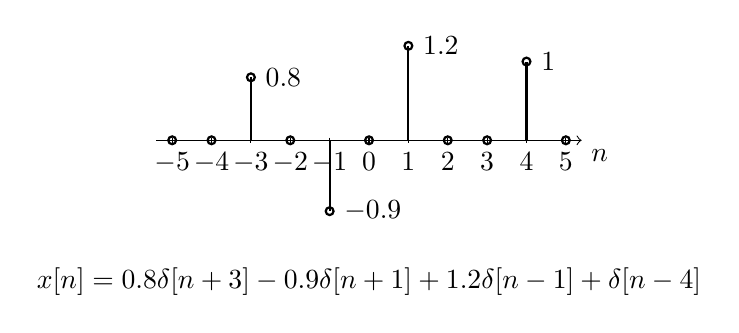
\begin{tikzpicture}
    \node[below,font=\bfseries] at (0,-1.5) {$x[n] = 0.8\delta[n+3] -0.9\delta[n+1] + 1.2\delta[n-1] + \delta[n-4]$};
    \draw[->] (-2.7,0) -- (2.7,0) node[anchor=north west] {$n$};
    \draw[thick] (-1.5,0) -- (-1.5,0.8);
    \draw[thick] (-.5,0) -- (-.5,-0.9);
    \draw[thick] (.5,0) -- (.5,1.2);
    \draw[thick] (2,0) -- (2,1);

\foreach \x in {-5,-4,...,5}
    \draw (\x*0.5 cm,1pt) -- (\x*0.5 cm,-1pt) node[anchor=north] {$\x$};

    \node [draw,inner sep=1pt, circle, thick](A) at (-2.5,0){};
    \node [draw,inner sep=1pt, circle, thick](B) at (-2.0,0){};
    \node [draw,inner sep=1pt, circle, thick,label=right:{$0.8$}](C) at (-1.5,0.8){};
    \node [draw,inner sep=1pt, circle, thick](D) at (-1.0,0){};
    \node [draw,inner sep=1pt, circle, thick,label=right:{$-0.9$}](E) at (-.5,-0.9){};
    \node [draw,inner sep=1pt, circle, thick](F) at (0,0){};
    \node [draw,inner sep=1pt, circle, thick,label=right:{$1.2$}](G) at (.5,+1.2){};
    \node [draw,inner sep=1pt, circle, thick](H) at (1,0){};
    \node [draw,inner sep=1pt, circle, thick](I) at (1.5,0){};
    \node [draw,inner sep=1pt, circle, thick,label=right:{$1$}](J) at (2,1){};
    \node [draw,inner sep=1pt, circle, thick](K) at (2.5,0){};
\end{tikzpicture}
\end{center}

In the above example, the se\-quen\-ce $x[n]$ is represented by a weighted sum of $\delta$ impulses $A\delta[n-\tau]$ with amplitude $A$ having the same value of the original se\-quen\-ce at the sample with position $-\tau$ from the origin.


\section{The sampling process}

Usually, when dealing with discrete-time se\-quen\-ces, one encounters examples of signals that are obtained by uniformly sampling a countinuous-time signal. In such scenario, one has a se\-quen\-ce $x[n]$ extracted from a signal $x_a(t)$ by means of a sampling process.

The relationship between the original con\-ti\-nuo\-us-time signal and the discrete-time se\-quen\-ce is the following one,
\[
    x[n] = x_a(t)\Bigr\rvert_{t=nT} = x_a(nT), n = \dots,-2,-1,0,1,2,\dots
\]
The above relationship between the original signal and the sampled se\-quen\-ce states that the sampling process is equivalent to simply pick the value of the countinous-time signal $x_a$ at \emph{some} samples $nT$. By performing such operation, one will obtain a sampled se\-quen\-ce with sampling period T$T$.

The time variable $t$ of the con\-ti\-nuo\-us-time signal $x_a(t)$ is related to the time variable $n$ of $x[n]$ only in some discrete-time instants $t_n$ that must abide to the following rule,
\begin{equation}\label{eqn:timeSamplingRule}
    t_n = nT = \frac n F_T = \frac {2\pi n} {\Omega_T},
\end{equation}
with $F_T = \frac 1 T$ denoting the sampling frequency, as expected. Indeed, $\Omega_T = 2\pi F_T$ is the \emph{sampling angular frequency}, in a constant multipliation-factor relationship between the sampling frequency.

Let's now consider the con\-ti\-nuo\-us-time sinusoidal signal
\[
    x_a(t) = A\cos{(2\pi f_0 t + \varphi)} = A\cos{(\Omega_0 t + \varphi)}
\]
and perform a sampling process with sampling period $T$. The resulting se\-quen\-ce will be
\begin{align}
    x[n] &= A\cos{(\Omega_0 n T + \varphi)} = A\cos{(\underbrace{\frac{2\pi \Omega_0}{\Omega_T}}_{\omega_0} n + \varphi)}, \\
         &= A\cos{(\omega_0 n + \varphi)},
\end{align}
where the angular frequency $\omega_0 := 2 \pi \frac {\Omega_0} {\Omega_T} = \Omega_0 T$ is the \emph{normalized digital angular frequency} of the se\-quen\-ce $x[n]$. Notice that an analog function generates \emph{different} sampled se\-quen\-ces according to the choice of the sampling period $T$. Indeed, \emph{different} sine functions can generate \emph{the same} sampled se\-quen\-ce if a peculiar $T^*$ is selected.

\subsubsection{Measurement units}

Measurements units are the following ones,
\begin{itemize}
    \item $T$ measures in seconds;
    \item $\omega_0$ in radians/sample;
    \item $\Omega_0$ in radians/second;
    \item analog frequency $f_0$ measures in hertz (Hz).
\end{itemize}

\subsection{Aliasing}

Let's pick three examples of con\-ti\-nuo\-us-time signals,
\begin{align*}
    g_1(t) &= \cos{(6\pi t)}, \\
    g_2(t) &= \cos{(14\pi t)}, \\
    g_3(t) &= \cos{(26\pi t)},
\end{align*}
of frequencies---respectively---of $3$Hz, $7$Hz and $13$Hz. Sampling the three signals at a sampling rate of $10$Hz, with $T=0.1s$, three se\-quen\-ces are soon generated,
\begin{align*}
    g_1[n] &= \cos{(0.6\pi n)}, \\
    g_2[n] &= \cos{(1.4\pi n)}, \\
    g_3[n] &= \cos{(2.6\pi n)},
\end{align*}

as $f_0 \cdot T = \frac{1}{10}f_0$.

Now, since
\begin{align*}
    g_1[n] &= \cos{(0.6\pi n)} =\\
           &= \cos{((2\pi - 0.6\pi)n)} = \cos{(1.4\pi n)} = g_2[n], \\
    g_1[n] &= \cos{(0.6\pi n)} =\\
           &= \cos{((2\pi + 0.6\pi)n)} = \cos{(2.6\pi n)} = g_3[n],
\end{align*}

all three se\-quen\-ces result to be identical. Therefore, it is rather difficult---let alone possible---to associate a unique con\-ti\-nuo\-us-time function with each of these se\-quen\-ces.

The phenomenon for which a con\-ti\-nuo\-us-time signal of high\-er frequency acquires the identity of a sinusoidal se\-quen\-ce of lower frequency after sampling is called \textbf{aliasing}. Since there are an infinite number of con\-ti\-nuo\-us-time signals that can lead to the same se\-quen\-ce when sampled periodically, additional conditions are needed so that the se\-quen\-ce $\{x[n]\} = \{x_a(nT)\}$ can uniquely represent the parent con\-ti\-nuo\-us-time signal $x_a(t)$. Indeed, in the above case $x_a(t)$ can still be fully recovered from the se\-quen\-ce $\{x[n]\}$. The process of bringing the angular frequency to a value between $0$ and $\pi$ is the \emph{normalization of the angular frequency}, a step that should always be performed as it is in the best interests to uniquely represent a specific class of sinusoids with a normalized representation.

Of course, there are many examples of se\-quen\-ces from which signals might be fully recovered. Suppose one wants to obtain the following discrete-time signal $v[n]$ from a con\-ti\-nuo\-us-time signal of shape
\begin{align*}
v_a(t) &=6\cos{60\pi t} + 3\sin{300\pi t} + 2\cos{340\pi t} \\ & + 4\cos{500\pi t} + 10\sin{660\pi t}
\end{align*}

with sampling period $T = \frac 1 {200} = 0.005s$.
To do so, one should perform the following algebraic transformations,
\begin{align*}
    v[n] &= 6 \cos{0.3 \pi n} + 3 \sin{1.5 \pi n} + 2 \cos{1.7 \pi n} \\
         &+ 4 \cos{2.5 \pi n} + 10 \sin{3.3 \pi n},\\
         &= 6 \cos{0.3 \pi n} + 3 \sin{(2\pi -0.5 \pi) n} + 2 \cos{(2\pi - 0.3\pi)n} \\
         &+ 4 \cos{(2 \pi + 0.5\pi) n} + 10 \sin{(4 \pi - 0.7\pi) n},\\
         &= 6 \cos{0.3 \pi n} - 3 \sin{0.5 \pi n} + 2 \cos{0.3\pi n} \\
         &+ 4 \cos{0.5\pi n} - 10 \sin{0.7\pi n},\\
    v[n] &= 8 \cos{0.3 \pi n} + 5 \cos{(0.5 \pi n + 0.6435)} - 10 \sin{0.7\pi n}.
\end{align*}

In the end, $v[n]$ is composed of 3 discrete-time sinusoidal signals of normalized angular frequencies $0.3\pi$, $0.5\pi$ and $0.7\pi$.

However, that's not the only signal possible that is capable of generating that very same sequence. Veritably, also the two following signals $w_a(t)$ and $g_a(t)$
\begin{align*}
    w_a(t) &= 8 \cos{60 \pi t} + 5\cos{(100 \pi t + 0.6435)} - 10\sin {140\pi t}\\
    g_a(t) &= 2 \cos{60 \pi t} + 4\cos{100 \pi t} + 10\sin {260\pi t}\\
           &+ 6\cos{460\pi t} + 3 \sin{700\pi t}
\end{align*}
will produce the very same sequence $v[n]$.

To avoid aliasing, an \emph{anti-aliasing} strategy should be adopted. As \textbf{Nyquist Sampling Theorem} dictates, since $\omega_0 = \frac{2\pi \Omega_0}{\Omega_T}$, if $\Omega_T > 2\Omega_0$ the corresponding normalized digital angular freqyency $\omega_0$ of the discrete-time signal obtained by sampling the parent continuous-time sinusoidal signal will be in the range $-\pi < \omega < \pi$, and no aliasing phenomena would occur. 

In practice, it is sufficient to select a sampling angular frequency $\Omega_T$ that is \emph{at least the double} of the $\Omega_0$ angular frequency of the sinusoid. On contrary, if $\Omega_T < 2\Omega_0$ the normalized digital angular frequency will fall in the range $-\pi < \omega < \pi$, then it will fold over a lower digital frequency $\omega_0 = \langle \frac{2 \pi \Omega_0 }{\Omega_T}\rangle_{2\pi}$ because of the aliasing phenomenon. This will inevitably lead to artifacts, as the sequence can be interpreted as different sinusoids other than the original one.

\subsubsection{Generalization}

Let's consider an arbitrary continuous-time signal $x_a(t)$, composed of a weighted sum of an arbitrary, finite number of sinusoidal signals. The signal might be uniquely represented---completely avoiding the aliasing effect---by a sequence $\{x[n]\}$, a sampled version of the original signal $x_a(t)$ with sampling frequency $\Omega_T$ that should be \emph{greater than the double of} the highest frequency in the signal $x_a(t)$. For instance, suppose $x_a$ contains a sinusoid whose frequency $f_h$ is the highest of all sinusoids in $x_a$; in order to avoid the aliasing effect, a correct choice for the angular sampling frequency would be $\Omega_T > 2\pi f_h$.
